\begin{center}
\section{Literature Review: Travelling Salesman Problem} \label{lit}
\end{center}

The Travelling Salesman Problem(TSP) is two problems in graph theory: a decision and an optimisation problem\cite{Cook1971}. However, it is most famous for its optimisation version, which is what this report covers. The most basic version of the optimisation problem is finding the shortest Hamiltonian cycle from a set of nodes(vertices) with non-negative weighted edges(links) to every other node(complete graph)\cite{Flood1956}. This can be formalised in graph theory with ordered pairs \(G = (V, E)\)\cite{Dantzig1954}.

\begin{itemize}
  \item \(G\), a graph
  \item \(V\), a set of nodes
  \item \(E\subseteq \{\{x,y,w\}\ |\ x,y\in V, w\in \mathbb{R}_{\geq0},  x \neq y\}\), a list of weighted edges from node x to node y
  \label{graph_data}
\end{itemize}

\begin{figure}[!ht]
    \centering
    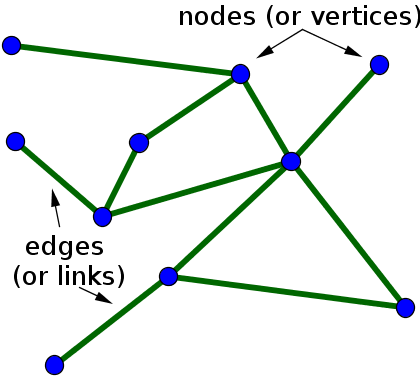
\includegraphics[scale=0.8]{sections/image/small_undirected_network_labeled.png}
    \caption{Graph Theory Diagram}
    \cite{Graph-Theory-Image}
\end{figure}


A Hamiltonian cycle is defined as from a graph, \(G =(V, E)\), an ordered list of edges creating a continuous path where every node is visited exactly once\cite{biggs1986graph}. In the research for TSP, the route can be defined as a 2-dimensional adjacency matrix, $A_{ij}$, of boolean values to represent if an edge is present in the cycle\cite{Croes1958}; It can also be listed as an ordered list\cite{Michael1970}, $P_i$,  where \(P\subseteq E\). The cost function of the cycle and the Travelling Salesman Problem is the summation of all the weights of the edges in the list \(P\) and is what is trying to be minimised\cite{Flood1956}:

\begin{equation}
    \min_{i \in P}(\sum \text{weight(}P_i))
    \label{TSPcost}
\end{equation}

Hamiltonian cycle has some formal constraints in graph theory\cite{biggs1986graph}:

\begin{itemize}
  \item \(|V| \geq 3\), There must be at least three nodes to create a cycle
  \item \(|P| = |V|\), The list must have as many edges as there are nodes in the graph
  \item \(\forall P_i: y_{i} = x_{i+1} \), Each edge in the list must create a continuous path
  \item \(\forall P_i \forall P_j:\ i\neq j, \ x_i \neq x_j, \ y_i \neq y_j\), Each node can only have two edges connecting to it in the route
\end{itemize}

\begin{figure}[H]
    \centering
    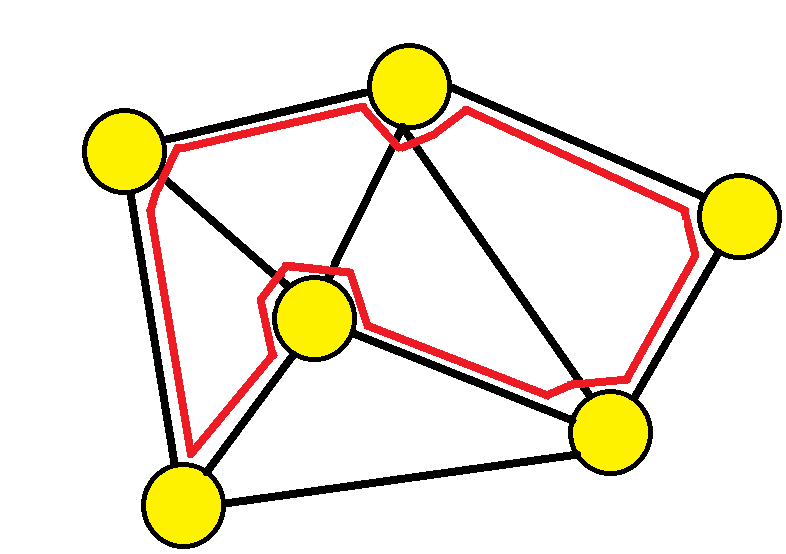
\includegraphics[scale=0.4]{sections/image/Hamiltonian.png}
    \caption{Hamiltonian Cycle}
    \cite{Hamiltonian-Path-Image}
\end{figure}

\label{hamiltonian-data}
While the adjacency matrix is more common in research, an ordered list is more memory efficient when programmatically storing a route. The list can store a list of edges or the order in which the nodes are visited. The latter is more popular as it is more memory efficient, but has slower read times. This is possible because the graph must be fully connected, therefore, the taken edges can be deduced from the adjacency matrix(Figure\ref{fig:adj}).

\begin{figure}[H]
    \centering
    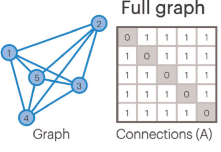
\includegraphics[scale=0.8]{sections/image/509624_1_En_15_Fig2_HTML.png}
    \caption{Adjacency Matrix}
    \label{fig:adj}
    \cite{Adjanceny-matrix-diagram}
\end{figure}

%\subsection{Versions Of Travelling Salesman Problem}
Over the years, constraints and variants of the classic optimisation problem have been conjured to fit the specific needs of researchers. Most are derived from changes to the type of graph the problem is solving\cite{Variants-tsp}: symmetric, asymmetric, Euclidean, Manhattan, two dimensions, three dimensions, and many more. But there are also new constraints like Dubins TSP\cite{Dubins-tsp}, which specifies that the route has a minimum turning radius, or K-TSP\cite{jiang2019algorithmsadaptivitygapsstochastic}, which introduces a starting hub and $k$ number of salesman/routes, or TSP with Time Windows(TSPTW)\cite{LOPEZIBANEZ20133806}, which adds temporal constraints to the problem.

\begin{figure}[!ht]
    \centering
    \begin{minipage}{0.45\textwidth}
        \centering
        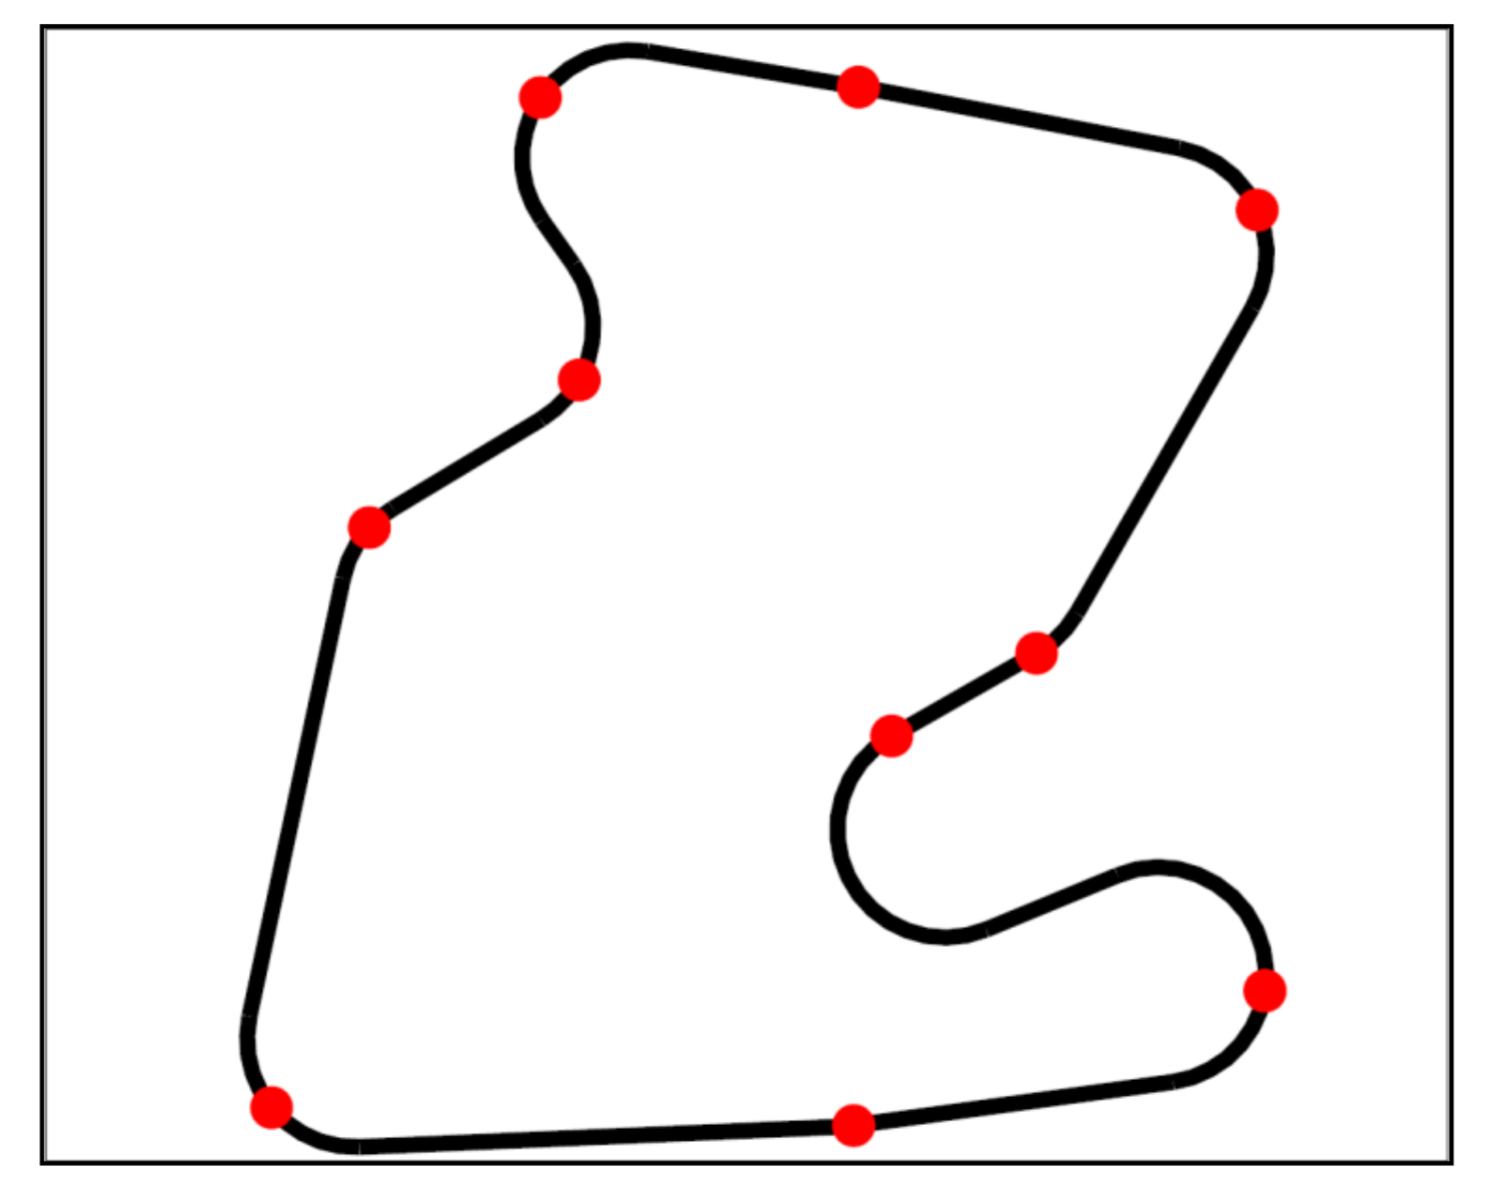
\includegraphics[width=0.9\textwidth]{sections/image/dtsp.png}
        \caption{Dubins TSP}
        \cite{dubins-tsp-picture}
    \end{minipage}\hfill
    \begin{minipage}{0.45\textwidth}
        \centering
        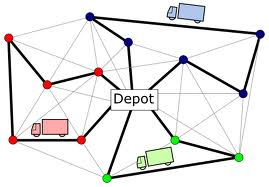
\includegraphics[width=0.9\textwidth]{sections/image/k-tsp.jpeg} % second figure itself
        \caption{K-TSP}
        \cite{K-tsp-picture}
    \end{minipage}
\end{figure}

A popular version is the symmetric two-dimensional Euclidean Hamiltonian Travelling Salesman Problem, which is used for the project for its adaptability to other problems. This is the most basic version and can be a catalyst for many other problems. It can be broken down into:
\begin{itemize}
  \item Edges between two nodes that have the same weight bidirectionally
  \item Nodes are positioned on a two-dimensional plane
  \item The distance between nodes is calculated using a straight distance
  \item The route is made up of only one Hamiltonian cycle
\end{itemize}

The TSP optimisation problem belongs to the NP-Hard classification of problems\cite{TSP-NP-hard}, as no algorithm exists for creating or verifying a solution in polynomial time. This is verifiable because there is a polynomial time reduction from the Hamiltonian cycle problem to the Travelling Salesman Problem\cite{CARMESIN2023102156}. All variants of TSP are also NP-Hard, as a polynomial-time reduction exists to handle the additional constraints\cite{Dubins-np-hard}.

When developing routes from nothing, two sub-procedures are used to generate a TSP solution. The different procedure determines if the algorithm is a tour constructor, a tour optimiser algorithm, or both\cite{Christian-tsp}. Tour constructor algorithms focus on adding unvisited nodes to a route in an optimal manner\cite{Rosenkrantz2009}. Tour optimiser algorithm focuses on improving an existing route by alternating the edges being taken\cite{tour-optimisation-paper}. The two sub-procedures are:
\vspace{0.5cm}
\begin{center}
    \begin{minipage}{0.8\linewidth}
        \begin{itemize}
            \item Construction: Iteratively adds an unvisited node to the route.
            \item Pairwise Exchange\cite{Englert2014}: Removing two edges from a route and reconnecting the resulting segments in an alternate way that still forms a cycle.
        \end{itemize}
        \captionof{table}{Sub-Procedures}
        \label{twosubprocedure}
    \end{minipage}
\end{center}
\vspace{0.5cm}
When geometric graphs are used, the Hamiltonian cycle has a property that the optimal solution will never have two edges that intersect each other due to the triangle inequality\cite{JEROMIN198970}. In Euclidean geometry, the triangle inequality states that the length of any two sides of a triangle is always greater than or equal to the length of the remaining side. Therefore, when a route is treated as a polygonal chain, a closed polygonal chain that does not form any triangles is strictly better than a polygonal chain that self-intersects and forms a triangle\cite{Kalmanson_1975}; this is the basic principle 2-opt is built upon.

\begin{figure}[H]
    \centering
    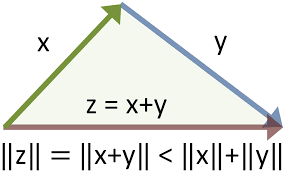
\includegraphics[scale=0.5]{sections/image/triangular_inequaility.png}
    \caption{Triangular Inequality}
    \cite{triangle-inequality-picture}
\end{figure}

\subsection{Exact Solution}
An exact or optimal solution is the route with the global minimum cost for a given graph; no other valid route has a lower cost\cite{Flood1956}. A graph can have multiple exact solutions if two or more routes have equal costs\cite{Capelli_2018}. An exact solution to the TSP is ideal in most situations, but it is sometimes a requirement in areas of research, such as DNA sequencing\cite{LEE200439}.

For a graph with \(n\) nodes, there are \(O(n!)\) possible routes\cite{Woeginger2003}. A simple approach to finding the optimal route would be a brute-force search, which calculates every possible combination of routes and stores the best result. This was taught in the year three Algorithms and Complexity module. However, with \(O(n!)\) possible routes and \(O(n)\) time to calculate the route cost, this becomes computationally infeasible after \(n\geq \approx20\)\cite{neoh2020evaluation}, due to exponential time growth\cite{Brute-Force}.

A similar mathematical problem is the sequencing problem\cite{Sequencing-problem}, which has an arbitrary cost function and a recurring scheme; this matches the TSP brute-force search. A dynamic programming solution exists for the sequencing problem\cite{DP-Sequencing} and can be applied to brute-force search\cite{TSP-DP}, which can cut down on the number of routes that need checking to \(O((n-1)2^{n-2})\)\cite{TSP-DP}. This is a significant improvement, but still means that problems after \(n\geq \approx57\) are infeasible.
\begin{figure}[H]
    \centering
    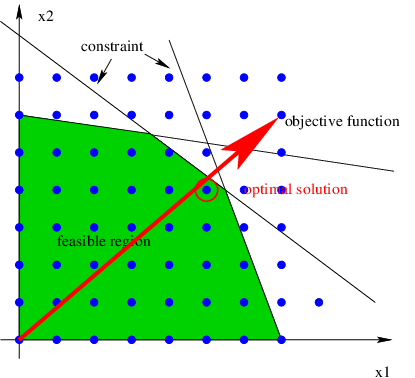
\includegraphics[scale=0.6]{sections/image/Example-Integer-Linear-Program-ILP.png}
    \caption{ILP Problem}
    \cite{ILP-diagram}
\end{figure}
Another method, not covered in the Algorithms and Complexity module, for solving exact solutions is solving TSP as an Integer Linear Programming(ILP) problem\cite{ILP}. ILP is an NP-hard optimisation problem with an objective function and a set of linear equations that must be satisfied. Some of these linear equations are developed from the definitions and constraints stated at the start of Section\ref{lit}. The worst-case time complexity for ILP is $O(n!)$\cite{diaby2006tsp}, but it can be significantly lower, depending on the problem\cite{HOOS201487}(covered in Section\ref{Concorde}).

% \begin{figure}[H]
%     \centering
%     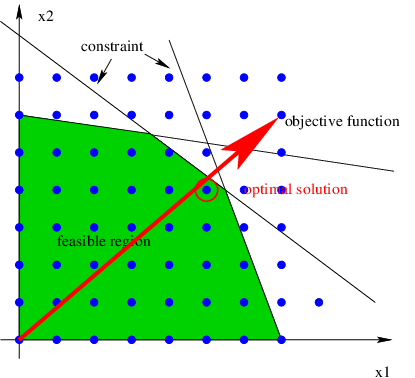
\includegraphics[scale=0.6]{sections/image/Example-Integer-Linear-Program-ILP.png}
%     \caption{ILP Problem}
%     \cite{ILP-diagram}
% \end{figure}

\subsubsection{Concorde TSP Solver}
\label{Concorde}
Due to the need for exact solutions to the Travelling Salesman Problem, research into optimising the development of exact solutions has been in development since the 1970s. William Cook, a researcher from the University of Waterloo, has made significant strides in this area over the past two decades with his team's Concorde TSP Solver\cite{concorde_tsp}, which is widely regarded as the best solver available\cite{HOOS201487}. Concorde holds the record for the largest TSP problem solved optimally at 85,900 nodes\cite{APPLEGATE200911} and is the first solver to obtain an exact solution to every problem in the TSPLib collection\cite{concorde_benchmarks}\cite{applegate2003implementing}, along with winning many awards for solving open problems\cite{amz_tsp}. It uses all of the most recent research and techniques, which this project researched and will explain.

Concorde is an extension of the University of Waterloo's research into solving Integer Linear Programming with their QSopt Linear Programming Solver\cite{APPLEGATE2007693}. Concorde solves problems by taking an existing good heuristic solution and relaxing the linear constraints to make the linear problem easier to solve\cite{applegate1998solution}. It can relax constraints using the Cutting-Plane Method, Branch-and-Bound, and Branch-and-Cut algorithms\cite{applegate2006traveling}.

\begin{figure}[H]
    \centering
    \begin{minipage}{0.45\textwidth}
        \centering
        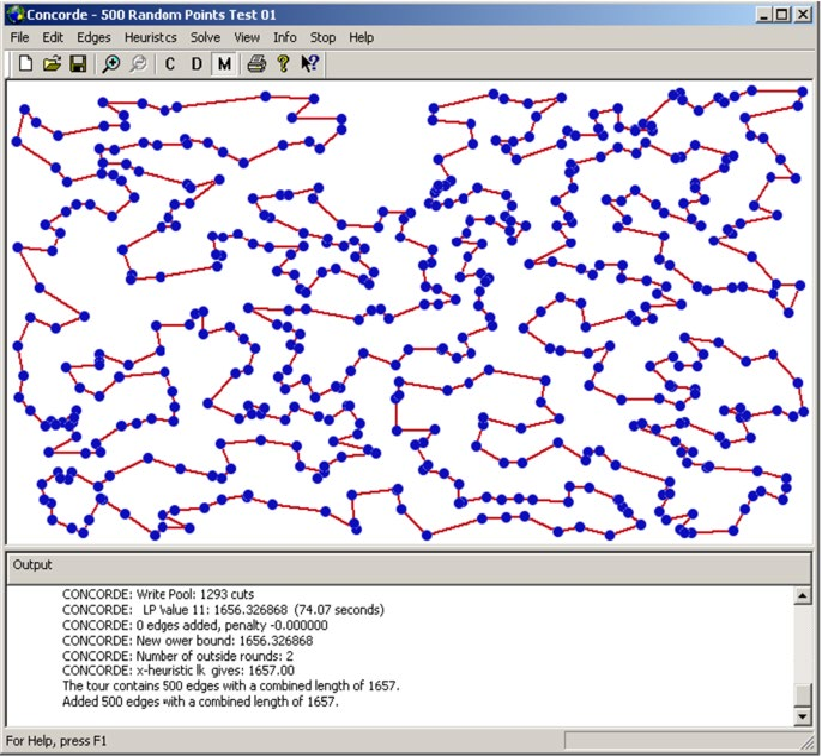
\includegraphics[width=\textwidth]{sections/image/Concorde-TSP-Solver-Solving-a-500-City-TSP-Instance.png}
        \caption{Concorde TSP Solver}
        \cite{concorde-picture}
    \end{minipage}\hfill
    \begin{minipage}{0.45\textwidth}
        \centering
        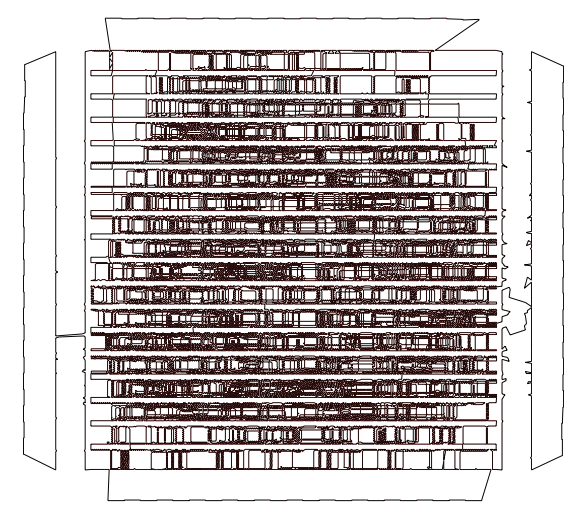
\includegraphics[width=\textwidth]{sections/image/85900_solution.png}
        \caption{85900 Node Solution}
        \cite{cook2012pursuit}
    \end{minipage}
\end{figure}

Branch-and-Bound(B\&B)(Figure\ref{fig:bab}) is an optimisation algorithm that solves Integer Linear Programming(ILP) problems by systematically branching the search space into smaller sub-problems and bounding non-promising branches\cite{MORRISON201679}. It achieves this by recursively dividing the solution space and using higher and lower bounds to eliminate sub-problems that cannot yield a better integer solution - a process known as ``pruning"\cite{VOLGENANT198283}. The best-known integer solution typically sets the upper bound, often obtained using TSP heuristic algorithms. In contrast, the lower bound is derived from solving relaxed Linear Programming(LP), where integer constraints are temporarily ignored\cite{APPLEGATE2007693}. This relaxed LP provides a bound that helps determine whether a branch should be explored further or pruned.

\begin{figure}[!ht]
    \centering
    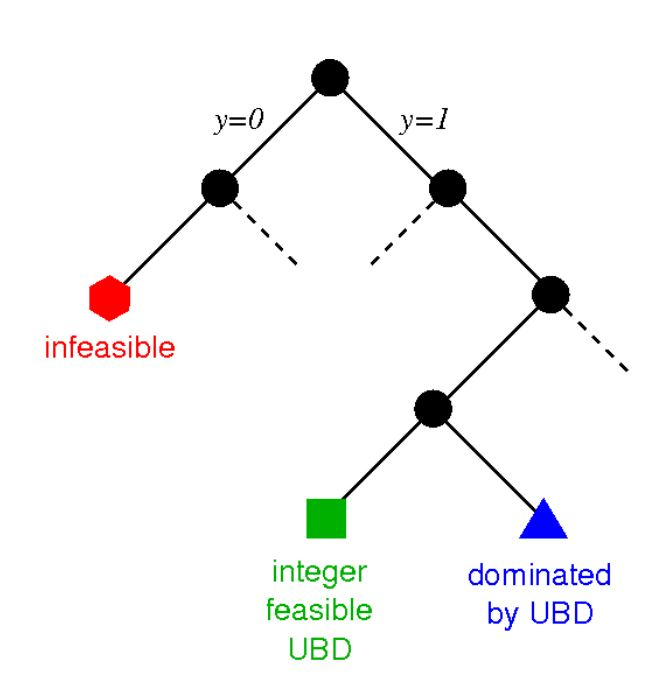
\includegraphics[width=0.5\textwidth]{sections/image/b&b.jpg}
    \caption{Branch And Bound}
    \label{fig:bab}
    \cite{cornell_bb_minlp}
\end{figure}


The Cutting-Plane Method(Figure\ref{fig:cutting}) is a technique for solving a Mixed-Integer Linear Program(MILP) by iteratively solving its Linear Programming(LP) relaxation and adding constraints(cuts) until an integer solution is found\cite{Cutting-plane}. First, it relaxes the problem to non-integer constraints and is solved as Linear Programming\cite{FLEISCHMANN1985307}. If the solution contains non-integer values, new hyperplanes(cuts) are added iteratively to the constraints until an integer solution is found\cite{applegate2003implementing}. The benefit of this approach is that LP is more straightforward to solve than MILP, but finding substantial cuts iteratively can be computationally expensive\cite{applegate2003implementing}.

\begin{figure}[H]
    \centering
    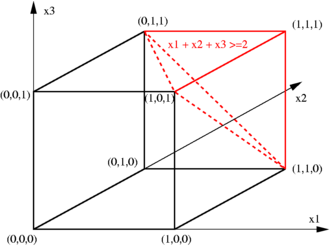
\includegraphics[width=0.6\textwidth]{sections/image/TSP_cutting_plane.png}
    \caption{Cutting-Plane Method}
    \cite{wikipedia_cutting_plane}
    \label{fig:cutting}
\end{figure}

Branch-and-Cut combines(Figure\ref{fig:bac}) Branch-and-Bound and Cutting-Plane methods into one\cite{mitchell2002branch}. It relaxes the problem to linear programming constraints, and in the pruning of Branch-and-Bound, it adds cuts back into the constraints. Added cuts can be global(cuts valid across the entire problem) or local(specific to a sub-problem in the search tree), and multiple branching strategies can be applied due to the relaxation\cite{branch-and-cut}. The benefit of Branch-and-Cut is its scalability for large-scale problems(\(n\geq\approx1000\))\cite{lu2022solvingclusteredtravelingsalesman}, making it the go-to approach for solving ILP.

\begin{figure}[H]
    \centering
    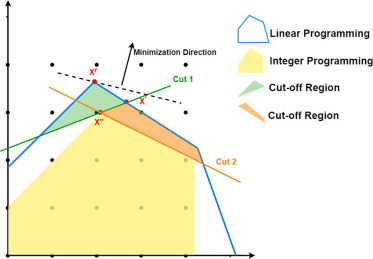
\includegraphics[width=0.6\textwidth]{sections/image/b&c.jpg}
    \caption{Branch And Cut}
    \label{fig:bac}
    \cite{ZHANG2023205}
\end{figure}

For Concorde TSP Solver, the efficiency is directly related to the starting solution provided, as it acts as the upper bound for Branch-and-Bound\cite{applegate2003implementing}. A tighter upper bound will reduce the number of valid branches by pruning more sub-problems. Therefore, research is still being applied to finding high-quality heuristics for the knock-on effect of finding a quicker exact solution in the Concorde TSP Solver.



Concorde's time complexity is not fixed because it depends on several factors, such as the starting heuristic solution and the specific instance of the problem\cite{applegate1998solution}. The worst-case complexity for branch-and-cut is exponential, \(O(2^n)\) \cite{John1963}, but practical performance is often significantly better, with standard hardware able to achieve \(n\geq\approx1000\) \cite{applegate2006traveling}. However, many software engineering optimisations are applied to hasten the solution time, allowing massive problems to be solved on supercomputers.

\subsection{Greedy Tour Construction Heuristic}

Sometimes, an approximate solution to the TSP is adequate for users when time complexity or computational resource constraints are a concern\cite{desale2015heuristic}. Amazon delivers approximately 1.6 million packages daily, with the average driver making 180 stops on their shift. This poses a logistical problem when a package could be out for delivery within a shorter time frame than the time to produce an exact solution. Another case is that many real-time path-finding applications must decide within seconds and are often limited by embedded hardware. Therefore, reliance on approximations for quick but quality solutions is still desirable for specific applications.

Heuristics are problem-solving strategies that use educated guesses to find approximate solutions quickly\cite{kokash2005introduction}. Heuristics are algorithms that follow structured logical steps; however, these logical steps take shortcuts, often trading completeness for speed. Greedy algorithms are a type of heuristic that makes local optimal choices to approximate global optimal solutions\cite{Jungnickel2013}; they are susceptible to pitfalls that cannot be solved later\cite{BANGJENSEN2004121}.

For the Travelling Salesman Problem, developing a route from a problem requires a construction strategy; these strategies are called tour constructions\cite{Christian-tsp}. A tour can be constructed in many ways and produce different results based on the starting location and variables. It usually starts with an empty route and randomly selects a node as the starting location; however, more innovative beginnings are available\cite{Christian-tsp}. Most tour constructors will iteratively add one node that is not already in the route to the route at the `head' or anywhere along the route.

Greedy tour constructors typically have polynomial time complexity and a fixed time complexity due to their exhaustive searching characteristics. Further improvements, such as caching and partitioning, can expedite the runtime, but the time complexity will remain the same. There are no guarantees on the lower bound of the solution cost against the optimal solution\cite{Vazirani2001}, as we would need to solve the P versus NP problem\cite{Vazirani2001}, which remains unproven.

\subsubsection{Nearest Neighbour}

The Nearest Neighbour Search(NNS) greedy algorithm is one of the oldest and most straightforward approaches for approximating the TSP. It was taught in the Algorithms and Complexity module. The origin of the heuristic is uncertain, but due to its simple nature, its approach is the most logical when thinking of a new method. The steps for the algorithm are as follows\cite{Nearest-neighbour}\cite{Rosenkrantz2009}:

\begin{legal}
  \item Select a random node as head and add it to the list of visited nodes
  \item Check every unvisited node:
  \begin{legal}
      \item select the unvisited node that has the lowest cost to the head
  \end{legal}
  \item Make the selected node the new head and add it to the list of visited nodes
  \item Repeat step 2 until there are no unvisited nodes
  \item Close the cycle by adding an edge from the current head to the starting node
\end{legal}

The time complexity for nearest neighbour is \(O(n^2)\)\cite{Christian-tsp}. It does \(n-1\) iterations from step 2 to step 4, and each iteration checks \(O(n)\) nodes as a possible shortest addition.

\subsubsection{Cheapest Insertion Heuristic}
\label{CIH}
The Cheapest(sometimes called shortest) Insertion Heuristic(CIH) takes a slightly more logical approach to constructing tours and was researched for this project. The addition of nodes to the route, can be added anywhere into the route\cite{Rosenkrantz2009}. The insertion cost formula for CIH calculates the breaking of the current route edge and the addition of two new edges. As nodes are added anywhere into the route, the starting route does not just have to be a single node; more advanced setups, such as Convex Hull\cite{Christian-tsp} or Shrinking Blob\cite{Jones2014}, can be adopted to improve the result\cite{jones2013computationtravellingsalesmanproblem}.

The insertion cost formula, where \(d(a,b)\) is the cost of the edge between node $a$ and $b$, \(x\) is the node to be added and \(a,b\) are consecutive nodes already in the route\cite{Rosenkrantz2009}:

\begin{equation}
    \text{Cost}(x,a,b) = d(x,a) + d(x,b) - d(a,b)  
    \label{CIH_Cost}
\cite{CIH}
\end{equation}

The steps for the algorithms are as follows\cite{CIH}\cite{Rosenkrantz2009}:

\begin{legal}
  \item Generate a starting route(random node or convex hull)
  \item For each unvisited node,
    \begin{legal}
        \item For every position in the route
        \begin{legal}
            \item Calculate the cost function of adding the node to the route position
        \end{legal}
    \end{legal}
  \item Add the selected node in the position with the lowest cost function
  \item Repeat step 2 until there are no unvisited nodes
\end{legal}

The time complexity for the cheapest insertion is \(O(n^3)\)\cite{Christian-tsp}. Its run-time changes based on the size of the starting route, but at worst, \(n-1\) iterations are run from steps 2 to 4. Each iteration is \(O(n^2)\), as \(O(n)\) unvisited nodes must calculate the cost function against \(O(n)\) positions in the route. Also, calculating the cost function(Equation\ref{CIH_Cost}) is three times more expensive than the Nearest Neighbour cost function, making CIH a significantly slower algorithm. 

\subsubsection{Convex Hull}

Convex Hull is a tour construction algorithm that does not guarantee a complete solution; instead, it generates part of a route\cite{MEERAN1997737}. The idea of a Convex Hull is to encapsulate all the points of a problem within a shape known as a convex hull\cite{lay1982convex}. Convex hulls utilise geometric locational properties of nodes, so only n-dimensional TSP problems based on Euclidean or Manhattan distance are suitable for using Convex Hulls\cite{MEERAN1997737}. 

\begin{figure}[!ht]
    \centering
    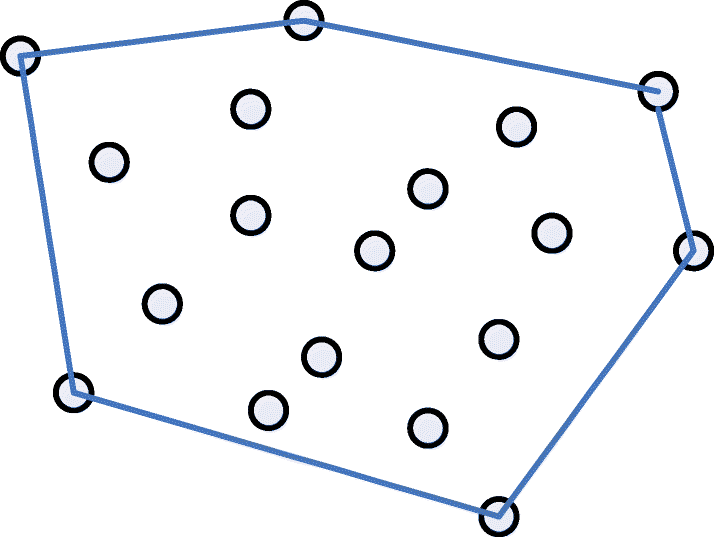
\includegraphics[width=0.4\textwidth]{sections/image/Convexhull.png}
    \caption{Convex Hull}
    \cite{Convexhull-picture}
\end{figure}


There are many algorithms for generating the structure, like Gift wrapping\cite{borgwardt1997average}, Graham scan\cite{GRAHAM1972132}, and Chan's Algorithm\cite{Chan1996}. Gift wrapping is the simplest to understand but the least efficient; the steps are\cite{borgwardt1997average}:

\begin{legal}
  \item Find the northernmost point, add it to the route, and make it the head
  \item For every node not in the route calculate the gradient to the head
  \item Add the node that forms the smallest counter-clockwise turn to the route and make it the new head
  \item Repeat step 2 until the head is back to the starting node
\end{legal}

The number of iterations is not fixed per problem, so \(h\) defines how many nodes are in the convex hull; \(h\) can be any size between \(n\geq h \geq 3\). Each time \(h\) increases by one, every node needs to be compared. Therefore, the gift-wrapping algorithm has a worse time complexity of \(O(n^2)\), but there exist more complex algorithms that run in \(O(nlog(n))\)\cite{GRAHAM1972132}.

The benefit of doing a Convex Hull is that it is a strong starting point for other heuristics\cite{MEERAN1997737}. The order of the nodes in a Convex Hull is guaranteed to be in the order of the optimal solution, as any other order of the partial route would have to cross over itself. This improves the results produced and quickens other tour constructors by reducing the number of nodes that need to be added. Algorithms that use Convex Hull address it in the name by placing it in the front, e.g. Convex Hull Cheapest Insertion Heuristic(CHCIH). This is because algorithms like CHCIH perform significantly better than CIH just by changing the starting route. 

\subsection{Existing Look-Ahead Solution}
\label{Look-ahead}

Look-ahead algorithms are valuable for dealing with decision problems\cite{murthy1995lookahead}; they are prevalent in tree searching and constraint solving\cite{frost1995look}. The premise is to evaluate future outcomes before making a decision by analysing future states to guide decision-making\cite{DongLookahead}. Look-ahead algorithms are not known for their speed, as additional computation power is required to evaluate future states, but they make up for it with above-average results\cite{SARKAR19941}. Research for look-ahead in TSP focuses primarily on adapting decision problems to different versions of TSP that can leverage this research\cite{Lin1973}.

\subsubsection{Nearest Neighbour Look-Ahead}
\label{NN-Look-ahead}
A paper by the Indian Institute of Technology called ``Improving Greedy Algorithms by Lookahead-Search"\cite{SARKAR19941} researches the use of look-ahead for solving the 0/1 Knapsack problem\cite{martello1990knapsack}. It is an optimisation decision problem for finding the optimal subset of items that maximises a cost function within a given constraint. The researchers devised that the decision problem can be formulated as a tree that can be recursively traversed to a look-ahead depth of $k$ with existing greedy algorithms\cite{SARKAR19941}. A tree structure is used because if it reaches a leaf node, then a constraint has been reached, and the algorithm should return. The researchers included pseudocode that worked for any generic greedy algorithm where the problem could be displayed as a tree\cite{SARKAR19941}.

\floatname{algorithm}{Algorithm}
\renewcommand{\algorithmicrequire}{\textbf{Input:}}
\renewcommand{\algorithmicensure}{\textbf{Output:}}

\begin{algorithm}[H]
\caption{lookahead-search$(k : \text{integer}, T : \text{tree}, G : \text{greedy algorithm})$}
\begin{algorithmic}[1]
\State $n : \text{node}$
\Comment{$k$-depth lookahead search in $T$ using $G$ as the underlying greedy algorithm.}
\State $path := \emptyset$
\State $n := \text{root}(T)$
\State lookahead$(k, n, G)$
\State print $path$ as the solution
\end{algorithmic}
\cite{SARKAR19941}
\end{algorithm}

\noindent Where Procedure \textit{lookahead} is defined recursively as follows:

\bigskip

\begin{algorithm}[H]
\caption{lookahead$(k : \text{integer}, n : \text{node}, \text{Greedy} : \text{greedy algorithm})$}
\begin{algorithmic}[1]
\State $l, m : \text{node}$
\If{$n$ is a leaf node}
    \Return
\Else
    \State Get $m \in \text{des}(n, k)$ such that
    \State \(
    \text{cost}(n \rightarrow m) + \text{Greedy}(m) = \min_{l \in \text{des}_{n, k}} \left\{ \text{cost}(n \rightarrow l) + \text{Greedy}(l) \right\}
    \)
    \State $m := \text{succ}(n \rightarrow m)$
    \State $path := path + \langle n, m \rangle$ \Comment{augment path; path is global}
    \State lookahead$(k, m, \text{Greedy})$
\EndIf
\end{algorithmic}
\cite{SARKAR19941}
\end{algorithm}

The researchers applied this pseudocode to the nearest neighbour greedy algorithm because it can be easily applied to a tree structure. The head node is the root state, and the greedy algorithm can be applied recursively to generate the states of the children nodes.

The researchers found that only minor improvements were made when applying the look-ahead design, however, it can produce better results than its greedy algorithm counterpart\cite{SARKAR19941}.

\subsubsection{Dubins Look-Ahead TSP Solver}

A paper by Automation Science and Engineering, titled ``Discretization-Based and Look-Ahead Algorithms for the Dubins Traveling Salesperson Problem" \cite{Cohen2017}, investigates the use of look-ahead for solving the Dubins version of the TSP. Dubins Travelling Salesman Problem(DTSP) adds the constraint that the route has a minimum turning radius\cite{Dubins-tsp}; this is to mimic the constraint that something like a fixed-wing aircraft faces.

The researchers developed a look-ahead algorithm for DTSP, where L is the look-ahead depth\cite{Cohen2017}:

\begin{legal}
  \item Get a solution for a corresponding Euclidean TSP
  \item Selected a random node as the head, $h$, and generate an initial heading to $h+1$ 
  \item Iterate $h$ for all nodes in the solution
  \begin{legal}
    \item Brute force calculates the shortest Dubins route for the subset, $h-1$ to $h+L-2$ nodes, where the heading of $h-1$ is fixed
    \item Permanently set the heading of $h$
  \end{legal}
  \item Return the newly organised solution
\end{legal}

The look-ahead part of this algorithm involves brute-forcing a small subset of the route and setting only the heading of node $h$. $h-1$ heading has to be fixed to allow for the continuous build-up of a Dubins route. Brute forcing a subset of the problem does not result in an exact solution because faults are introduced in the combination step, but it does provide a better result than if a greedy approach were taken.

%\subsubsection{Beam Search Heuristic}

%A paper by Yuan Ze University called ``A Beam Search Heuristic for the Traveling Salesman Problem with Time Windows" researches the use of look-ahead for solving the TSP with Time Windows(TSPTW). TSPTW introduces a temporal constraint for when a node can be visited, this is found in networking problems.

%Beam Search is a modification on the breadth-first search of trees by pruning the number of nodes that are tracked at each layer to a value, $\beta$. As fewer nodes are evaluated at each layer, it saves on memory and computational power by only choosing the most potential nodes via estimations. However, the results of the pruning are dependent on how accurate the estimations are.

%The researchers proposed a few Beam Search techniques for TPSTW with Local evaluation, Global evaluation, and implementation details of the evaluation. Each uses partial routes(the beam nodes) and different ways of iteratively inserting which node. For Local Evaluation, it generates all nodes to a depth $L$ and creates a cost function(weighs route length, time weight violations).

\subsection{Tour Optimisation Heuristic}

Sometimes, the initially constructed route is not good enough, and simple improvements can be made to the route's ordering to achieve a better result \cite{Christian-tsp}. This is where Tour Optimisation algorithms are used to improve the ordering and refine the edges taken from an already complete cycle while maintaining the properties of the TSP\cite{Christian-tsp}.

Tour Optimisation heuristics effectively resolve local pitfalls that have been taken, but they struggle to find global pitfalls. Optimisers rarely find the exact solutions to a problem, but they are valuable as they often find improvements on existing solutions cheaply. This report researches its design.

\subsubsection{2-opt}

The simplest optimisation heuristic is Croes's 2-opt local search algorithm in 1958\cite{Croes1958}. It utilises the property that any two edges crossing over each other are suboptimal and calculates whether swapping edges can produce a better result. For Symmetric graphs, the cost function below calculates if swapping two edges will benefit the route:

\begin{equation}
    Cost(r_i,r_j) = d(r_i,r_j) + d(r_{i+1},r_{j+1}) -d(r_i,r_{i+1}) - d(r_j,r_{j+1})
\cite{Englert2014}
\end{equation}

The steps for 2-opt are as follows\cite{Croes1958}:

\begin{legal}
    \item For each pair of edges $(i, j)$, where $i$ ranges from $0$ to $n-1$ and $j$ ranges from $i+2$ to $n$:
    \begin{itemize}
        \item Calculate the cost of swapping the edges.
        \item If the swap results in a negative cost, perform the swap.
    \end{itemize}
    
    \item Repeat step 1 until no swaps result in a negative cost.
\end{legal}

The time complexity of 2-opt is often difficult to predict in real-world examples, as it is unknown how many iterations it will perform. Each iteration takes \(O(n^2)\)\cite{Englert2014}, as it checks two nested For loops of combinations. Although 2-opt is likely to converge after only a few iterations, the worst-case scenario is \(O(n^2)\) iterations due to the numerous combinations of swaps available for an edge before it reaches a location it has been in before. Therefore, the worst case for 2-opt is \(O(n^4)\)\cite{Englert2014}, however if applying a limit of $m$ iterations results in \(O(m\cdot n^2)\). 

\subsection{Software Engineering Optimisation}
\label{SWEOps}
When solving the TSP, the fundamentals of each algorithm remain the same, but data structures and algorithms can be applied to achieve a constant-factor speed-up. Each software engineering optimisation benefits the computational runtime for the average case, but the Big O time complexity remains the same in the worst case\cite{applegate2006traveling}. 

\subsubsection{Caching}
\label{lit:Caching}
Caching is the process of storing computational results to be used later for quick callback. When the problem is assigned as a list of nodes, the edge weights are not necessarily known at run time\cite{applegate2006traveling}. Calculating edge weights can be expensive depending on the TSP problem type(3D Euclidean, Global Coordinates, A* Pathfinding)\cite{Caching-performance}. Therefore, a 2D Adjacency Matrix can store $n^2$ edge results. Two fill strategies can be applied to deal with caching:

\begin{itemize}
    \item Full: Calculate every edge weight before trying to solve the problem
    \item Partial: See if the edge weight has been cached before; if not, calculate the edge
\end{itemize}

If it is known that an algorithm will scan most edges, doing full caching is ideal, as there is no overhead for checking if a cache miss has occurred. If an algorithm does not scan all the edges, partial caching helps reduce unnecessarily expensive calculations.

\subsubsection{Partitioning}
\label{partitioning}
Partitioning is the process of bucketing nodes into groups based on the geometric location of the point\cite{applegate2006traveling}. There are two use cases for partitioning in the Travelling Salesman Problem\cite{karp1977probabilistic}\cite{Clustering-Tsp}\cite{Partioning-tsp}\cite{lin2022grid}:

\begin{itemize}
    \item Closeness proximity: Reduce the search size of nodes based on proximity
    \item Creating smaller problems:
        \begin{enumerate}
            \item Group sets of nodes together
            \item Solve each set
            \item Merge the solutions to solve the original problem
        \end{enumerate}
\end{itemize}

Closeness proximity is helpful when evaluating potential nodes in heuristics\cite{Partioning-tsp}; it can cheaply exclude nodes as valid options. The partitioning algorithm's search time is typically $O(log(n))$; therefore, reducing the search space usually results in an expedited solution without affecting the result.

Splitting a large problem into smaller problems can be useful as time complexity grows exponentially\cite{karp1977probabilistic} with problem size. By dividing the problem, each solution becomes more manageable, but the solution quality drops as decision boundaries are formed between the smaller problems, resulting in disjointed routing\cite{lin2022grid}. It is merging of solutions step that introduce imperfections in the solution quality\cite{tsp_subproblems}.

There are many partitioning algorithms, but the most common are K-means Clustering\cite{k-means}, Grid-based\cite{arora1998polynomial}, and Quad-Trees\cite{arora1998polynomial}.

\begin{itemize}
    \item K-means Clustering: Given $k$ clusters; distribute each cluster such that the nodes are evenly grouped between the clusters
    \item Grid-based partitioning: Split the graphing area into evenly distributed quadrilaterals and bucket the nodes to them
    \item Quad-Trees: Subdivides the graphing area into smaller and smaller quadrilaterals in a quad-tree structure; nodes are assigned at each layer of the tree
\end{itemize}

K-means clustering is expensive to calculate and progressively more complex as the number of clusters increases\cite{k-means-2}. However, many clusters are beneficial when partitioning the TSP problem, and K-means struggles when there is an even distribution of points\cite{k-means}.

\begin{figure}[H]
    \centering
    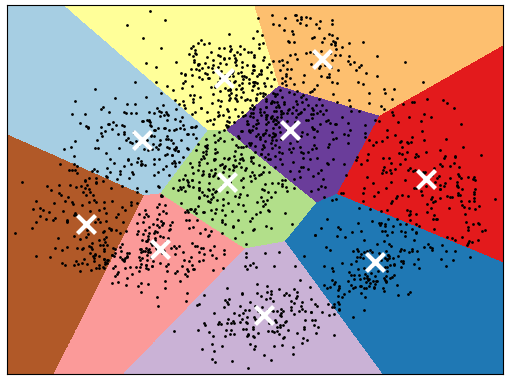
\includegraphics[width=0.65\textwidth]{sections/image/k-means.png}
    \caption{K-Means Partitioning}
    \cite{scikit-learn-kmeans-example}
\end{figure}

Grid-based partitioning is the most straightforward approach with the quickest search and creation times and works well for evenly distributed points. When the points are concentrated, grid-based partitioning fails to separate the points by grouping a large number of points in the same bucket.

\begin{figure}[H]
    \centering
    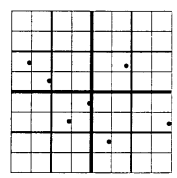
\includegraphics[width=0.4\textwidth]{sections/image/Grid-based.png}
    \caption{Grid-based Partitioning}
    \cite{arora1998polynomial}
\end{figure}


Quad-tree partitioning takes a hierarchical approach by subdividing the problem based upon the points\cite{samet1984quadtree}. As each point is assigned its own node in the tree, testing for closeness can be more precise, and the results are better for densely packed nodes\cite{arora1998polynomial}. However, the construction is expensive\cite{samet1984quadtree}, there is an overhead in search time\cite{samet1984quadtree}, and it requires a significant amount of memory.

\begin{figure}[H]
    \centering
    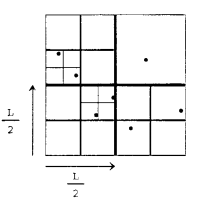
\includegraphics[width=0.4\textwidth]{sections/image/Quad-tree.png}
    \caption{Quad-Tree Partitioning}
    \cite{arora1998polynomial}
\end{figure}

\begin{table}[!ht]
\centering
\begin{tabular}{|l|l|l|l|}
\hline
\multicolumn{1}{|c|}{{ \textbf{Partitioning}}} & \multicolumn{1}{c|}{{ \textbf{Creation Time}}} & { \textbf{Read Time}} & { \textbf{Partitioning Result}} \\ \hline
K-Means                                           & O(2nki)                                           & O(1)                     & Average                                 \\ \hline
Grid-Based                                        & O(n)                                              & O(1)                     & Worst                                 \\ \hline
Quad-Tree                                         & O(nlog(n))                                        & O(log(n))                & Best                               \\ \hline
\end{tabular}
\end{table}

Although partitioning has many benefits, it requires the data to have geometric properties. The benefits are also not guaranteed, especially when the nodes are densely packed.

\subsubsection{Parallelisation}

Parallel computing involves splitting calculations across multiple processors and executing them simultaneously\cite {Parallel-computing}. There are many challenges, mainly related to data handling and synchronisation\cite{Navarro_Hitschfeld-Kahler_Mateu_2014}. But the Travelling Salesman Problem lends itself well to parallelisation due to the iterative nature of finding the best fit and only changing the problem state once all options have been considered\cite{KINDERVATER1989249}. Parallelisation is how cutting-edge technology like Concorde TSP Solver can solve massive problems using supercomputers\cite{applegate2003implementing}.

GPUs can also be applied to TSP algorithms\cite{applegate2003implementing} due to their capabilities in matrix arithmetic and vectorisation programming. Two 2D Adjacency Matrices are multiplied together, and the grand sum is taken to calculate the length of the route, allowing for quick calculations. Researchers tested the speed difference for a few algorithms and recorded a dramatic reduction in run-time of 24.2 times quicker than their CPU counterparts\cite{GPU}.